\documentclass[../main.tex]{subfiles}
\graphicspath{
    {"../img/"}
    {"img/"}
}

\begin{document}
    \subsubsection{dodatek na temat kąta}
    Było
    \[
        \sin(\sphericalangle \dot{z}, \bar{z})
    .\]
Ma być
\[
    \begin{vmatrix} x &\dot{x}\\ y & \dot{y} \end{vmatrix} = |z| |\dot{z}| \sin\left( \sphericalangle(z,\dot{z}) \right)
.\]
\subsubsection{Powrót do residuów w nieskończoności}
Dostaliśmy na Wykładzie 18
\[
    a_n = - \frac{2}{2 \pi i} \int\limits_{\substack{\partial K(0,t)\\ t > \frac{1}{r}}} f(z) z^{n-1}dz
.\]
Wielkość
\[
    - a_1 = - \frac{1}{2\pi i}\int\limits_{\substack{\partial K(0,t)\\ t > \frac{1}{r}}}f(z) dz
\]
nazywamy residuum funkcji $f$ w nieskończoności.
\begin{stw}
    Niech $f$ - holomorficzna na $\mathbb{C}$ z wyjątkiem punktów $z_1,\ldots,z_k$, ale $z_i$ - biegun $p_i$ rzędu (nie ma punktów istotnie osobliwych). Wówczas
    \[
    \sum_{\Res f + \Res \infty}f = 0
    .\]
\end{stw}
\begin{proof}
    Niech $z_i$ takie, że
    \[
    \underset{A}{\exists} \quad \underset{i}{\forall}\quad z_i\in A
    .\]
Wówczas
\[
    -\int\limits_{\partial A}f + \sum_i\int\limits_{\partial K(z_i,r_i)} = 0
.\]
\end{proof}
\begin{pytanie}Jak obliczyć $a_1$?\end{pytanie}
    Zauważmy, że gdy rozwiniemy
    \[
        g(z) = f\left(\frac{1}{z}\right)
    \]
    w szereg Laurenta wokół zera, to $g(z)$ przyjmuje postać
    \[
        g(z) = \ldots + \frac{a_{-2}}{z^2} + \frac{a_{-1}}{z} + a_0 + a_1z + a_2z^2 + \ldots
    .\]
Zauważmy, że
\[
    \frac{g(z)}{z^2} = -\frac{a_{2}}{z^4} + \frac{a_{-1}}{z^3} + \frac{a_0}{z^2} + \frac{a_1}{z} + a_2 + \ldots
.\]
Zatem
\[
    \underset{\infty}{\Res} f(z) = - \underset{0}{\Res} \frac{f\left( \frac{1}{z} \right) }{z^2}
.\]
\begin{przyklad}
    \[
        \int\limits_{|z| = 2}\frac{dz}{(z^8 + 1)^2} = \sum\limits_{\underset{(-1)}{\Res} \frac{1}{8}} f = - \underset{\infty}{\Res} f(z)
    .\]
Ale
\[
    f(z) = \frac{1}{(z^8 + 1)^2}
.\]
\[
    g(z) = f\left( \frac{1}{z} \right) = \frac{1}{\left( \left( \frac{1}{z} \right) ^8 + 1 \right) ^2} = \frac{z^{16}}{(1 + z^8)^2}
\]
    i liczymy $\underset{0}{\Res}\quad \frac{g(z)}{z^2}$
    Ale
    \[
        \lim\limits_{z\to 0}\frac{z\cdot z^{14}}{(1+z^8)^2} = 0
    .\]
Więc całka też $0$.
\end{przyklad}
\begin{figure}[h]
    \centering
    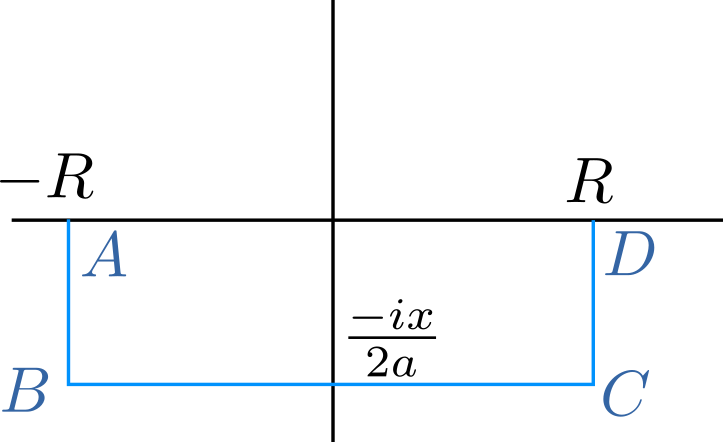
\includegraphics[width=0.3\textwidth]{w20-1}
    \caption{w20-1}
    \label{fig:w20-1}
\end{figure}
\begin{przyklad}
    Sytuacja jak na rys. \ref{fig:w20-1}
    \[
    J = \int\limits_{-\infty}^{+\infty}e^{ixt}e^{-at^2}dt,\quad a \ge 0
    .\]
\[
    J = \int\limits_{-\infty}^{+\infty}e^{-a\left[ (t - \frac{ix}{2a})^2 + \frac{x^2}{4a^2}\right]}dt = e^{-a\frac{x^2}{4a^2}}\int\limits_{-\infty}^{+\infty}e^{-a(t - \frac{ix}{2a})^2}dt
.\]
Liczymy teraz
\[
    \int\limits_{-\infty}^{+\infty}e^{-a\left( t - \frac{ix}{2a} \right)^2 }dt = \lim\limits_{R\to +\infty}\int\limits_{-R}^{+R}e^{-a\left( t - \frac{ix}{2a} \right) ^2}dt = \lim_{R \to +\infty} \int\limits_{-R - \frac{ix}{2a}}^{R - \frac{ix}{2a}}e^{-as^2}ds
.\]
Niech $f(z) = e^{-az^2}$
 \[
 \int\limits_{AB}f + \int\limits_{BC}f + \int\limits_{CD}f + \int\limits_{DA}f = 0
 .\]
 $BC$ już mamy, więc
    \[
    \int\limits_{BC}f = -\int\limits_{DA}f - \int\limits_{BA}f - \int\limits_{CD}f
    .\]
Pokażemy, że
\[
\lim_{R \to +\infty}\int\limits_{CD}f = 0
.\]
Parametryzacja $CD := \left\{ z = R + iy, -\frac{x}{2a}\le y \le 0 \right\} $
\[
    \int\limits_{CD}f = \int\limits_{-\frac{x}{2a}}^{0}idy\cdot  e^{-a\left( R+iy \right) ^2} = i\int\limits_{-\frac{x}{2a}}^{0}dy\cdot e^{-aR^2}e^{-2Riya}e^{ay^2}
.\]
\[
\left| \int\limits_{CD}f \right| \le e^{-aR^2} \left| \frac{x}{2a} \right| \cdot \left| e^{-2Riya} \right| \cdot \underset{-\frac{x}{2a}\le y \le 0}{\max}  \left| e^{ay^2} \right| \underset{R\to \infty}{\longrightarrow} 0
.\]
I tak samo będzie z całką po $AB$. Jeszcze zostało $DA$
\[
\lim_{R \to +\infty}-\int\limits_{DA}f = \int\limits_{-\infty}^{+\infty}e^{-ax^2}dx = \sqrt{\frac{\pi}{a}}
.\]
Zatem
\[
\int\limits_{-\infty}^{+\infty}e^{ixt}e^{-at^2}dt = \sqrt{\frac{\pi}{a}} e^{-\frac{x^2}{4a}}
.\]
\end{przyklad}
\subsection{Transtormata Fouriera}
\textbf{Obserwacja:} Rozwińmy $f(z)$ w $R(0,a,b)$, $a,b < 1$
\[
    f(z) = \sum_{n=-\infty}^{+\infty} a_nz^n
.\]
\[
    a_n = \frac{1}{2\pi i}\int\limits_{\substack{\partial K(0,t)\\ a < t < b}}\frac{f(z)}{z^{n+1}}dz
.\]
Wstawmy $z = e^{ix}$
 \[
     g(z) = f\left(e^{ix}\right) = \sum_{n=-\infty}^{\infty} a_n e^{mx}
 .\]
 Ale
 \[
     \frac{1}{2\pi i} \int\limits_{\partial K(0,t)}\frac{f(z)}{z^{n+1}}dz = \begin{matrix} z = e^{ix}\\ dz = ie^{ix}dx\end{matrix} = \frac{1}{2\pi i}i \int\limits_{0}^{2\pi} \frac{f\left( e^{ix} \right) }{e^{(ix)(n+1)}}e^{ix}dx
 .\]
 \[
     a_n = \frac{1}{2\pi}\int\limits_{0}^{2\pi}g(x)e^{-inx}dx
 .\]
 \begin{definicja}
     Transformatą Fouriera funkcji $f$ nazywamy wielkość
     \[
         \mathcal{F}(f)(x) \equiv \hat{f}(x) = \int\limits_{-\infty}^{+\infty} e^{-i2\pi xt}f(t)dt
     .\]
 \end{definicja}
 \textbf{Uwaga: }transformatę Fouriera możemy zdefiniować też tak
 \begin{definicja}
     (inne notacje)
     \[
         \hat{f}(x) = \frac{1}{\sqrt{m} }\int\limits_{-\infty}^{+\infty}e^{iq\sigma xt}f(t)dt
     ,\]
 gdzie $m = \left\{ 1,2\pi \right\} $, $q = \left\{ -1, 1 \right\} $, $\sigma = \left\{ 1,2\pi \right\} $.\\
     Konwencja u nas:
     \begin{itemize}
         \item $m = 1 $
         \item $q = - 1$
         \item $\sigma = 2pi$
     \end{itemize}
 \end{definicja}
 \begin{przyklad}
     \[
         f(x) = \begin{cases}
             1&|x|\le a\\ 0 & |x| > a
         \end{cases}
     .\]
 \begin{align*}
     \hat{f}(x) &= \int\limits_{-\infty}^{+\infty}f(t)e^{-i 2\pi t x}dt = \int\limits_{-a}^{+a}e^{-i 2\pi tx}dt = \left.-\frac{1}{2\pi i x}e^{-i 2 \pi t x}\right|_{-a}^{a} =\\
     &= -\frac{1}{2\pi i x}\left[ e^{-i 2 \pi a x} - e^{i 2 \pi a x} \right] = \frac{\sin(2\pi a x)}{\pi x}
 .\end{align*}
 Czyli jak na rys. \ref{fig:w20-2}
 \end{przyklad}
 \begin{figure}[h]
     \centering
     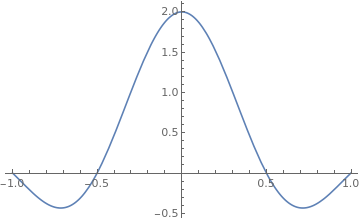
\includegraphics[width=0.6\textwidth]{w20-2}
     \caption{Wynik przefourierowania $f$}
     \label{fig:w20-2}
 \end{figure}
 \begin{definicja}
     Niech $f: \mathbb{R}\to \mathbb{R}$. Mówimy, że
     \begin{itemize}
         \item $f$ - klasy $L_1$, jeżeli
              \[
             \int\limits_{\mathbb{R}}|f| < +\infty
             .\]
     \item $f$ - klasy $L_2$, jeżeli
         \[
         \int\limits_{\mathbb{R}}|f|^2 < +\infty
         .\]
     \end{itemize}
 \end{definicja}
 \begin{przyklad}
     \[
         f(x) = \begin{cases}
             \frac{1}{^2\sqrt{x^3}} & 0 < x \le 1\\
             0 & \text{w p.p.}
         \end{cases}
     .\]
 \[
     g(x) = \begin{cases}
         \frac{1}{^2\sqrt{x^3} }& x > 1\\
         0 & \text{w p.p.}
     \end{cases}
 .\]
 Zbadać, czy $f$ jest klasy $L_1$ lub (i) $L_2$ i czy $g$ jest klasy $L_1$ lub (i) $L_2$
 \end{przyklad}

\end{document}
